\section{Keisler with Graph Neural Networks}

\subsection{Machine Learning Architecture}

\begin{figure}[ht]
\centering
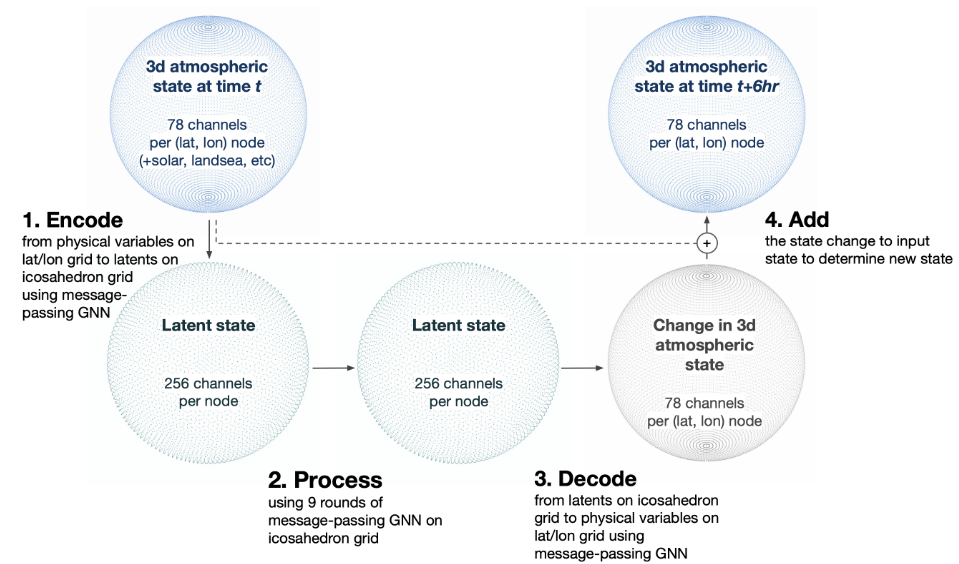
\includegraphics[width=0.9\textwidth]{media/Keisler_archi.png}
\caption{Keisler Model Learning Architecture}
\label{fig}
\end{figure}

The model employs Graph Neural Networks (GNNs) and is inspired by the approach of Pfaff et al. \cite{pfaff}. The GNN parameters are learned using historical training data (ERA5), leveraging the JAX library and two JAX-based packages: Jraph for constructing the GNN structures and Haiku for managing the neural networks themselves.

The model architecture is presented as follows: three main components - an encoder, a processor, and a decoder. The encoder maps the data from the native space (physical data on a latitude/longitude grid) to an intermediate space (abstract feature data on an icosahedral grid), while the processor handles this data in the intermediate space and the decoder maps the results back to the native space.

The use of an icosahedral grid for the intermediate representation is motivated by the fact that it provides a more uniformly distributed and efficient processing grid than the original latitude/longitude grid. The H3 package is used to define an icosahedral grid of level 2, which consists of 5,882 nodes (compared to 65,160 in the original lat/lon grid) with an angular separation of 3 degrees (approximately 330 km) between the nodes.

Each of the three components of the model is implemented as a message-passing GNN, using 2-layer MLPs with ReLU activation, LayerNorm, and 256 output channels for the neural networks.

\subsection{Data Availability}

All codes are available on this \href{https://github.com/openclimatefix/graph_weather/tree/main}{GitHub repository}.